\chapter{Exploration}\label{exploration}

\section{Survey \& Interviews}\label{survey-interviews}

To form a general understanding of how IDEs and some of their specific
features are used, an online survey targeted towards professional
developers was created. The survey ran in April 2014 over the course of
two weeks and yielded answers from 45 participants.

Besides general questions, e.g. which programming languages and IDEs the
participants used, it collected information about the usage of the
following IDE functionalities:

\begin{itemize}
\itemsep1pt\parskip0pt\parsep0pt
\item
  Navigation of code
\item
  Debugging
\item
  Usage of API and language documentation
\item
  Autocompletion
\item
  Project structure and scaffolding
\item
  Asynchronicity
\item
  Syntax Highlighting
\end{itemize}

For each of the areas it was asked if and how the participants were
using them and—if appropriate—how their IDE was supporting them. They
survey instrumented multiple-choice questions with an additional „Other“
field for custom answers, as well as open-ended questions with a
free-form text field.

\subsection{Survey Results}\label{survey-results}

\subsection{Interview Results}\label{interview-results}

\section{Solutions to analogous
problems}\label{solutions-to-analogous-problems}

The most ubiquitous visualization of program structure is probably
\textbf{syntax highlighting} or \emph{syntax colouring}. This concept
aims to makes the developer distinguish entities of the programming
language by showing them in different font types, weights, styles, or
colours. According to the survey results (see
section\textasciitilde{}\ref{survey-interviews}), syntax highlighting
can help with a number of different problems: recognizing errors and
typos, distinguishing language constructs from variables and values, and
orientation through specific visual patterns. In Figure
\ref{fig:syntaxhighlighting} that is showing syntax highlighting in an
HTML document, HTML elements are printed in blue, whereas attributes are
printed in purple, values in red, comments in yellow and content in
black.

\begin{figure}[htbp]
\centering
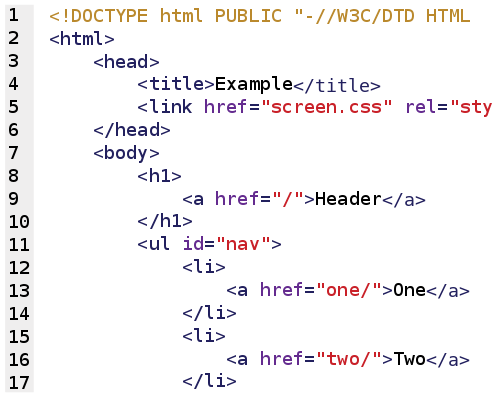
\includegraphics[keepaspectratio,width=0.75\textwidth,height=0.75\textheight]{img/syntax_highlighting.png}
\caption{Syntax highlighting in an HTML document}
\label{fig:syntaxhighlighting}
\end{figure}

In his talk „Monads and Gonads“, Douglas Crockford presents an
alternative to syntax highlighting which he calls \textbf{„context
colouring“} \citeyear{crockford}. Instead of using font styles and
colours in order to highlight different elements of the \emph{syntax},
he instead highlights different \emph{contexts}. Figure
\ref{fig:contexthighlighting} illustrates this concept: The global scope
is presented in white, whereas nested contexts are marked green, yellow
and blue, respectively. In this concrete example, identifiers are always
coloured in the colour of the context of \emph{where they were defined}.
For example, the appearance of \texttt{value} in the innermost context
is yellow, the colour of the scope in which \texttt{value} was declared
(as a function parameter to the function \texttt{unit}).

\begin{figure}[htbp]
\centering
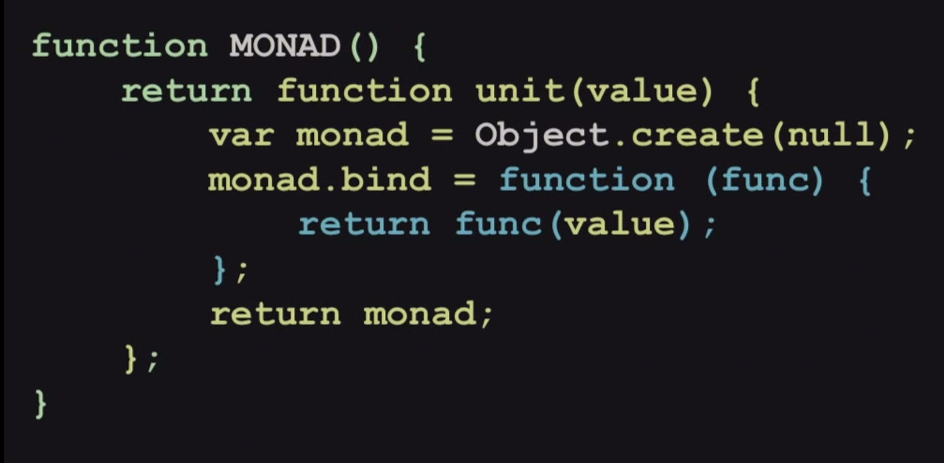
\includegraphics[keepaspectratio,width=\textwidth,height=0.75\textheight]{img/context.png}
\caption{Context colouring in JavaScript, as proposed by Crockford\footnote{Screenshot taken from \cite{crockford}}}
\label{fig:contexthighlighting}
\end{figure}

\textbf{Theseus} is a JavaScript debugger built as a plug-in for the
Brackets IDE. It makes use of the code editor itself and shows
information inline, in the gutter and in a panel on the bottom of the
Brackets window (see Figure \ref{fig:theseus}). Theseus is mostly used
for asynchronous debugging, so the way those UI elements are used
corresponds do this purpose. For every function definition, Theseus
shows the number the function has been called in the gutter. Functions
that have never been called are marked with a grey background in the
source code. Additionally, the panel on the bottom shows information
about the function the cursor is positioned in\footnote{It shows
  asynchronous call stacks, which are not of relevance to this thesis.}.

\begin{figure}[htbp]
\centering
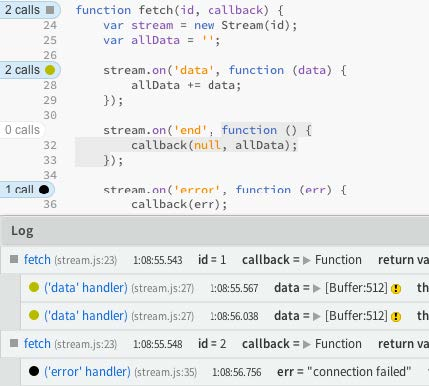
\includegraphics[keepaspectratio,width=0.75\textwidth,height=0.75\textheight]{img/theseus.jpg}
\caption{Theseus’ asynchronous JavaScript debugging \cite{lieber}}
\label{fig:theseus}
\end{figure}

\textbf{JSHint} is a so-called \emph{linting} tool for JavaScript: it
detects bad coding practices by checking JavaScript code against a set
of rules, and therefore tries to prevent common problems. Originally
built as a command-line tool and for online code checking, JSHint is
implemented in many IDEs through the respective plug-in systems. The
\emph{Sublime Linter} plug-in\footnote{See
  \url{http://www.sublimelinter.com/}} for Sublime Text 3 implements
JSHint (and other linting tools) \emph{inline}: hints of bad code or
inconsistent style are shown in the text editor itself and are indicated
in the gutter. If the cursor is on top of problematic code, the
respective hint is printed in the status bar.

(Sublime Linter screenshot)

In terms of navigating and displaying the scope and context information
in relation to the actual source code, the \emph{Element Inspector} of
\textbf{Chrome Developer Tools} makes a good example (see Figure
\ref{fig:devtools}). It shows the source code of the inspected website
and allows the user to select any \ac{html} element within. In the
remaining parts of the window, information relevant to the selected
element is shown.

\begin{figure}[htbp]
\centering
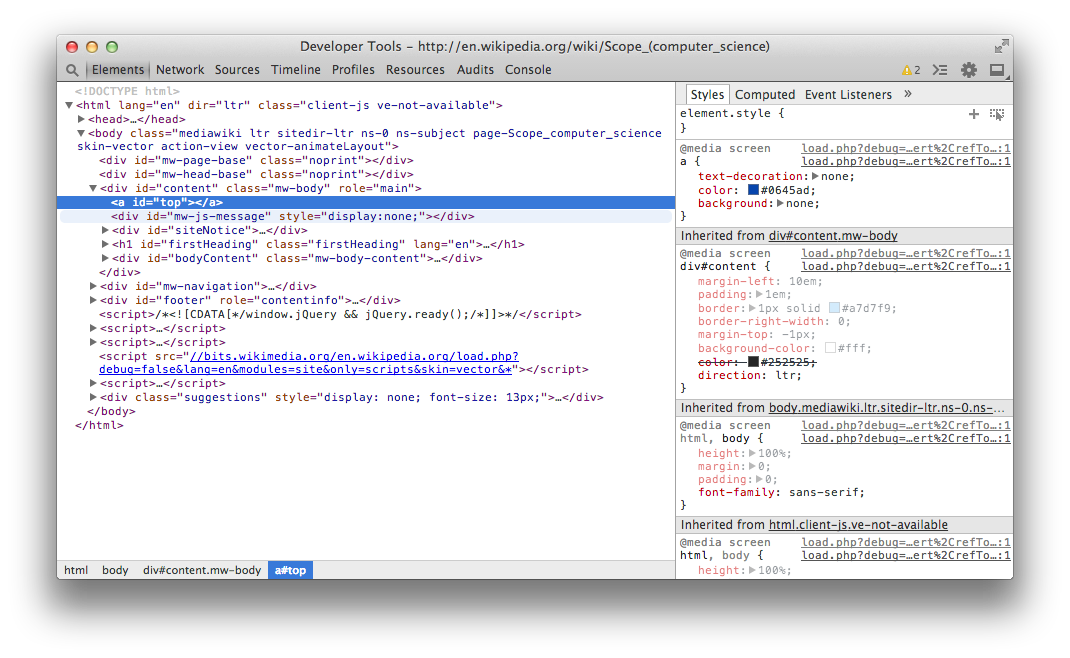
\includegraphics[keepaspectratio,width=\textwidth,height=0.75\textheight]{img/devtools.png}
\caption{Chrome DevTools with Element Inspector}
\label{fig:devtools}
\end{figure}

At the bottom of the window, a status bar shows the nesting of the
selected element: on top is the \texttt{html} element, inside it the
\texttt{body}, then a \texttt{div} and finally the selected \texttt{a}
element. This status bar can be used to navigate around the nested
elements by clicking on them. Clicking on the \texttt{body} element
highlights it in the source code as well, and shows different style
information on the right-hand side.

Place to the right of the source code is a sidebar. Although it contains
a tabbed interface to browse different facets of the selected element,
the one that is relevant is the one in focus on the screenshot,
\emph{Style}. The way style (through \ac{css}) is applied to HTML
elements is similar to the way nested scope works: style that is defined
on the containing elements may influence the style of the selected
elements, which is why the relevant styles are listed in order of
precedence. The style rules that apply with the highest precedence are
listed on top, while the rules with the least precedence are listed on
the bottom. Style rules that are overriden by rules of higher precedence
are marked by a line through the rule. This way of visualizing and
organizing information about nested structures is further used in the
following concept and design phases (see section {[}concepts{]} and
chapter {[}design{]}).

\section{Ideation}\label{ideation}

To support the ideation phase, the author created a collection of
existing UI components within IDEs. Those components were written down
on post-it notes.

The components were used a seeds for \emph{seeded brainstorming}: for
each of the components, the author tried to imagine solutions that are
similar, related to or based on the respective component.

Most of the ideas that came out of the brainstorming session made use of
multiple components, for example the \emph{context path} which is
described further down: it made use of a status bar as well as the code
editor.

Most of the ideas of the brainstorming phase made it into first
sketches. The sketching happened with two different approaches,
depending on if the code editor was involved or not.

For ideas that involved the code editor, it was important that the
author could work with real, functioning code. Therefore, two sample
JavaScript applications were created to work with:

\begin{itemize}
\itemsep1pt\parskip0pt\parsep0pt
\item
  A small web server application, that would parse a markdown-formatted
  text file and render it into an HTML template. The application would
  run on Node.js and represents a typical control flow for e.g. a
  blogging engine (content + template = site).
\item
  A client-side script (runs in a browser) that fetches JSON data and
  presents them on a website, by the click of a button. This script
  represents typical client-side UI code, connecting a button event to a
  function and presenting the result in the UI.
\end{itemize}

Both applications were written in different styles: the server-side
application decouples the different tasks by putting them into different
functions (as far as it makes sense), whereas the client-side
application nests all function definitions inside each other, resulting
in nearly one function definition in each line, and deeper indentation
(ergo: higher code complexity).

A good solution for this design problem should address both cases.

Printouts of the two JavaScript files served as a basis for ideation
\emph{within source code}.

For concepts that would mainly work with other UI components, such as a
sidebar, or such concepts that would introduce new UI components, blank
paper was used for sketching.

\section{Concepts}\label{concepts}

\begin{itemize}
\itemsep1pt\parskip0pt\parsep0pt
\item
  \emph{Context Path} - a path view of the context tree, similar to that
  of a selector path in an HTML editor (screenshot!). The context at the
  position of the cursor would be shown in a status bar. By hovering
  over a context level, the corresponding source code would be
  highlighted in the source editor.
\item
  \emph{Context Graph} - similar to a class browser, the context graph
  would represent a tree view of the application’s context(s). This
  could be implemented as a sidebar or panel.
\item
  \emph{Context Colouring} - similarly suggested by Crockford
  \citeyear{crockford}, the source code can be coloured in depending on
  its context (level). Crockfords variation is meant to replace syntax
  highlighting; one could, as well, complement syntax highlighting by
  colouring in the background (as e.g. Theseus does). 50 Shades of Grey.
\item
  \emph{Inspect Context} - comparable to DevTools’ \emph{Inspect
  Element} function, the user can right-click into the source code and
  choose \emph{Inspect Context}, which opens a panel that shows global
  variables, current local variables as well as the value of
  \texttt{this}.
\item
  \emph{Gutter Context} - any change of context or scope is indicated in
  the code editor’s gutter (similar to JSHint).
\item
  \emph{Quick Inspect} - similar to Brackets’ \emph{Quick Edit} feature,
  the value of \texttt{this} could be inspected inline.
\end{itemize}

http://ariya.ofilabs.com/2012/11/language-tools-for-reducing-mistakes.html
